\documentclass[12pt,reqno]{amsart}
\usepackage{./header, amssymb}

\hdr{Mathematical Statistics}{Chapter 12: Probabilistic graphical models}

\begin{document}

\bigskip

\prob Suppose that we have three binary random variables $X$, $W$, and $H$, which indicate whether a person exercises regularly ($X$), whether they are overweight ($W$), and whether they have heart disease ($H$). Discuss several causal structure involving these variables.

\bigskip
\textcolor{red}{We first might believe that $X$ is a confounding variable in the relationship between $W$ and $H$, meaning the causal graph has the form $W \leftarrow X \rightarrow H$. This means a person's decision to exercise has a direct influence on both their weight and whether they have heart disease, and that any statistical correlation between the latter variables is the result of this common cause and not a result of a direct cause and effect relationship between the two. Alternatively, we might believe that $X$ serves as a mediating variable between $W$ and $H$, meaning the causal graph has the form $W \to X \to H$. This means that a person's weight directly influences their decision to exercise, and then this latter decision directly influences whether they have heart disease. However, this causal model still assumes there is not a direct cause and effect relationship between $W$ and $H$.}
\bigskip













\prob Let $X$ and $Y$ be binary random variables that indicate whether a person has \textit{hydromechanical trepidation syndrome} ($X$) and whether they test positive ($Y$) for it. Suppose that
	\[p(y=1 |x=1) = 0.98 \quad \text{and} \quad p(y=1 | x=0) = 0.1.
	\]
Express the flow of information from $X$ to $Y$ as a stochastic link by explicitly writing down a link function.

\bigskip
\textcolor{red}{The link from $X$ to $Y$ is given by
	\[Y \mid X \sim \mathcal{B}er(\theta), \quad \theta = g(x) = 0.1(1-x) + 0.98x.
	\]}
\bigskip
	







\prob Explicitly draw the full graphical structure for a plated linear regression model

\bigskip
\begin{center}
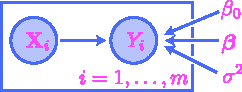
\includegraphics[scale=1.5]{lin-reg-00-plated.pdf}
\end{center}
\bigskip

when $m=3$.

\bigskip
\textcolor{red}{See your solutions from class.}
\bigskip













\prob Given a linear regression model with predictors $\mathbf{X}$, response $Y$, and parameters $\beta_0$, $\boldsymbol{\beta}$, and $\sigma^2$, we saw in class that
	\[ R \mid \mathbf{X} = \mathbf{x} \sim N(0, \sigma^2)
	\]
where $R = Y - \beta_0 - \mathbf{X}^\intercal \boldsymbol{\beta}$ is the error term. Prove this claim.

\bigskip
\textcolor{red}{Given $\mathbf{X} = \mathbf{x}$, we have
	\[R = Y - \beta_0 - \mathbf{x}^\intercal \boldsymbol{\beta},
	\]
where $Y \mid \mathbf{X} = \mathbf{x} \sim N(\mu,\sigma^2)$ with $\mu = \beta_0 + \mathbf{x}^\intercal \boldsymbol{\beta}$. This shows that $R \mid \mathbf{X} = \mathbf{x}$ is an affine transformation of a normal random variable, and so Theorem 5.7 applies to give us the desired result.}
\bigskip










\prob Compute the inverse of the sigmoid function $\sigma(x) = 1/(1+e^{-x})$. Interpret its meaning.

\bigskip
\textcolor{red}{Supposing $p = \sigma(x) = 1 / (1+e^{-x})$, easy algebra shows that the inverse function is given by
	\[x = \sigma^{-1}(p) = \log\left( \frac{p}{1-p} \right).
	\]
The ratio $p/(1-p)$ is often called the \textit{odds} of an event of probability $p$ occurring. If this event is drawn from a sample space with uniform probability measure, then it is simply the number of outcomes resulting in the event occurring, divided by the number of outcomes for which the event does not occur. Thus, the inverse function $\sigma^{-1}$ is often called the \textit{log-odds function}. (It is also sometimes called the \textit{logit function}.)}
\bigskip












\prob The \textit{confusion matrix} for the logistic regression model discussed in class is given by
	\[\begin{array}{c|cc}
	& \hat{y}=0 & \hat{y} = 1 \\ \hline
	y=0 & 422 & 90 \\
	y=1 & 95 & 417
	\end{array}
	\]
where $y$ is the true class and $\hat{y}$ the predicted class of an instance in the dataset. In this problem, a \textit{positive} class label corresponds to $1$, while a \textit{negative} class label corresponds to $0$.

\medskip
\begin{enumerate}
\item Compute the \textit{accuracy} of the classifier, which is the proportion of correctly classified instances out of all total instances.

\bigskip
\textcolor{red}{The accuracy is
	\[\frac{422 + 417}{1024} \approx 0.819.
	\]}
\bigskip

\item Compute the \textit{precision} of the classifier, which is the proportion of all true positive predictions out of all positive predictions. (High precision $=$ avoids false positives.)

\bigskip
\textcolor{red}{The precision is
	\[\frac{417}{90 + 417} \approx 0.822.
	\]}
\bigskip

\item Compute the \textit{recall} (or \textit{sensitivity}) of the classifier, which is the proportion of all true positive predictions out of all actual positive instances. (High sensitivity $=$ avoids false negatives.)

\bigskip
\textcolor{red}{The recall is
	\[\frac{417}{95 + 417} \approx 0.814.
	\]}
\bigskip

\item Discuss situations in which the primary interest is in classifiers with high precision, versus a situation in which the primary interest is high sensitivity.

\bigskip
\textcolor{red}{We would desire a spam filter to have high precision, since this means that it rarely tags a legitimate email as spam. (Where $1=$ spam and $0=$ not spam.) A high sensitivity is also desirable, since this means it avoids letting spam emails through to the user's inbox, but most users are willing to endure a stray spam email every now and then as long as the filter never misclassifies potentially important emails as spam. On the other hand, we would want an internet content filter to have high sensitivity. (Where $1=$ inappropriate and $0=$ appropriate.) This means that it would rarely mark inappropriate material as appropriate. A high precision is also desirable, since this means it avoids marking appropriate material as inappropriate, but most users are willing to endure a lower precision score as long as it means the filter never lets inappropriate content pass through which could lead to all sorts of very bad outcomes.}
\bigskip
\end{enumerate}








\prob Describe a possible neural network architecture for datasets of the form
	\[(\mathbf{x}_1,y_1),(\mathbf{x}_2,y_2),\ldots,(\mathbf{x}_m,y_m) \in \mathbb{R}^n \times \mathbb{R},
	\]
where the $y_i$'s are drawn from a continuous random variable $Y$.

\bigskip
\textcolor{red}{We may modify the architectures described in class by taking the output neuron to be distributed normally. For a neural network of depth $d$, the final link function is of the form
	\[Y \mid \mathbf{X} \sim N(\mu,\sigma^2) \quad \text{where} \quad \mu = \mathbf{a}_{d-1} ^\intercal \mathbf{w}_d + b_d.
	\]}

\end{document}